\documentclass{snapshotmfo}
\categorizationmath{algebra and number theory,analysis,discrete mathematics and foundations,geometry and topology,numerics and scientific computing,probability theory and statistics}
\categorizationconnect{chemistry and earth science,computer science,engineering and technology,finance,fine arts,humanities and social sciences,life science,physics,reflections on mathematics}
\license{CC-BY-SA-4.0}
\snapshotid{472}{1950}
\junioreditor{Some One}{junior-editors@mfo.de}
\senioreditor[f]{Anja Randecker}{senior-editor@mfo.de}
\director[m]{Gerhard Huisken}
\usepackage[utf8]{inputenc}
\usepackage{amsmath,amssymb}
\usepackage{longtable}

\usepackage[french]{babel}
\usepackage[french]{cleveref}

\author{Test Author}
\title{french cleveref}
\begin{document}
\pdfbookmark{french cleveref}{snapshottitle}

\begin{abstract}
Check, if the following cleveref names are french. Please note, that with french, colons don't seem to work in label names!
\end{abstract}

\noindent\begin{longtable}{@{}l@{\quad yields\quad}l@{}}
	\verb+\Cref{real}+             &\Cref{real}.\\
	\verb+\cref{real}+             &\cref{real}.\\[1ex]
	\verb+\Cref{chartwo}+           &\Cref{chartwo}.\\
	\verb+\cref{chartwo}+           &\cref{chartwo}.\\[1ex]
	\verb+\Cref{thm.continuity}+   &\Cref{thm.continuity}.\\
	\verb+\cref{thm.continuity}+   &\cref{thm.continuity}.\\[1ex]
	\verb+\Cref{tab.Jordan}+       &\Cref{tab.Jordan}.\\
	\verb+\cref{tab.Jordan}+       &\cref{tab.Jordan}.\\[1ex]
	\verb+\Cref{fig.Institute}+    &\Cref{fig.Institute}.\\
	\verb+\cref{fig.Institute}+    &\cref{fig.Institute}.\\[1ex]
	\verb+\Cref{fig.maya}+         &\Cref{fig.maya}.\\
	\verb+\cref{fig.maya}+         &\cref{fig.maya}.\\[1ex]
	\verb+\Cpageref{fig.maya}+     &\Cpageref{fig.maya}.\\
	\verb+\cpageref{fig.maya}+     &\cpageref{fig.maya}.\\[1ex]
	\verb+\Cref{sec.heading}+      &\Cref{sec.heading}.\\
	\verb+\cref{sec.heading}+      &\cref{sec.heading}.\\[1ex]
	\verb+\Cref{sec.another}+      &\Cref{sec.another}.\\
	\verb+\cref{sec.another}+      &\cref{sec.another}.\\[1ex]
	\verb+\Cref{subsec.first}+     &\Cref{subsec.first}.\\
	\verb+\cref{subsec.first}+     &\cref{subsec.first}.\\[1ex]
	\pagebreak
	\verb+\Cref{subsec.another}+   &\Cref{subsec.another}.\\
	\verb+\cref{subsec.another}+   &\cref{subsec.another}.\\[1ex]
	\verb+\Cref{subsubsec.sample}+ &\Cref{subsubsec.sample}.\\
	\verb+\cref{subsubsec.sample}+ &\cref{subsubsec.sample}.\\[1ex]
	\verb+\Cref{footnote}+         &\Cref{footnote}.\\
	\verb+\cref{footnote}+         &\cref{footnote}.\\
\end{longtable}


\section{A heading}
\label{sec.heading}
The cleveref package handles various types of labels enumerated independently of each other, e.\,g.
figures, tables, equations, sections, subsections, and subsubsections.
\verb+\cref{<labelname>}+ returns the labels together with their respective types {\em in the chosen language}.
See the cleveref package documentation for the full set of commands and options.

\begin{figure}[ht]
	\centering
	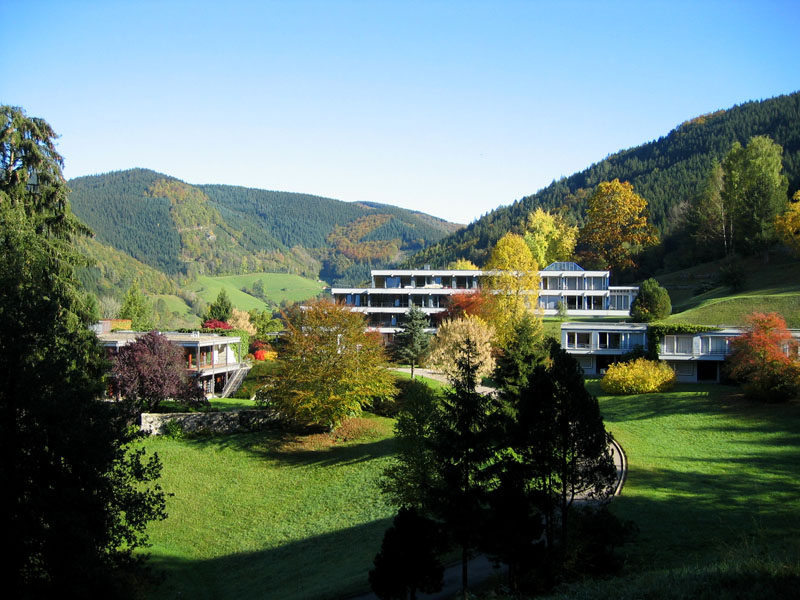
\includegraphics[width= 0.33 \textwidth]{mfo.jpg}
	\caption{An image scaled to 33\% of the textwidth.}
	\label{fig.Institute}
\end{figure}

\begin{table}[ht]
	\caption{Jordan canonical form}
	\begin{tabular}{ l c r }
		17 & 1 & 0 \\
		0 & 17 & 0 \\
		0 & 0 & -3 \\
	\end{tabular}
	\label{tab.Jordan}
\end{table}

\subsection{A subsection}
\label{subsec.first}
More text and some formulas:
\begin{align}\label{real}
	1+1&=2,\\\label{chartwo}
	1+1&=0.
\end{align}
Formula \eqref{real} refers to $\mathbb{R}$, Formula \eqref{chartwo} does not\footnote{This is a footnote.\label{footnote}}.


\section{Another section heading}
\label{sec.another}

\subsection{Another subsection} \label{subsec.another}

\begin{figure}[ht]
	\centering
	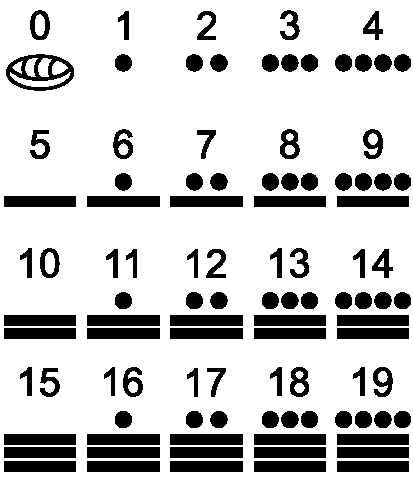
\includegraphics[width= 0.33 \textwidth]{maya.pdf}
	\caption{Exemplary image: Maya numerals.}
	\label{fig.maya}
\end{figure}

\subsubsection{Sample subsubsection} \label{subsubsec.sample}

\newtheorem{theorem}{Theorem}
\begin{theorem}\label{thm.continuity}
	Differentiability implies continuity.
\end{theorem}



\begin{imagecredits}
	\item[\Cref{fig.Institute}] Archives of the Mathematisches Forschungsinstitut Oberwolfach,\\\url{http://www.mfo.de}, 2004.
	\item[\Cref{fig.maya}] ``Maya''. Author: Bryan Derkson. Licensed under Creative Commons Attribution-Share Alike 3.0 via Wikimedia Commons, \url{http://commons.wikimedia.org/wiki/File:Maya.svg}, visited on \printdate{2014-09-05}.
\end{imagecredits}

\end{document}
